\documentclass{beamer}
  % Xe(La)TeX
  \usepackage{fontspec}
  \usepackage{xunicode}
  \usepackage{soul}
  \usepackage{eurosym}
  \usepackage{textcomp}

  % Style général
  \usetheme{Frankfurt}
  \usefonttheme{professionalfonts}
  \setbeamertemplate{navigation symbols}{}

  % Charte fédérale.
  \definecolor{blue}{HTML}{729FCF}
  \setbeamercolor{structure}{fg=blue}
  \setbeamercolor{block body}{bg=blue,fg=white}
  \setbeamercolor{block title}{bg=blue,fg=white}
  \setbeamercolor{block body alerted}{bg=blue,fg=white}
  \setbeamercolor{block title alerted}{bg=blue,fg=white}
  \setbeamercolor{block body example}{bg=blue,fg=white}
  \setbeamercolor{block title example}{bg=blue,fg=white}

  % Paquetages utiles.
  \usepackage[absolute,overlay]{textpos}
  \usepackage{etoolbox}
  \usepackage{tikz}

  % Compteur spécifique pour partager les numéros de page
  \newcounter{multipleslide}
  % Commande pour concerver le meme compteur de page
  \makeatletter%
  \newcommand{\multipleframe}{%
  \setcounter{multipleslide}{\value{framenumber}}
  \stepcounter{multipleslide}
  \patchcmd{\beamer@@tmpl@footline}% <cmd>
    {\insertframenumber}% <search>
    {\themultipleslide}% <replace>
    {}% <success>
    {}% <failure>
  }
  \newcommand{\restoreframe}{%
  \patchcmd{\beamer@@tmpl@footline}% <cmd>
    {\themultipleslide}% <search>
    {\insertframenumber}% <replace>
    {}% <success>
    {}% <failure>
  \setcounter{framenumber}{\value{multipleslide}}%
  }
  \makeatother%

  % Pied de page.
  \setbeamertemplate{footline}{
    \leavevmode%
    \hbox{\hspace*{-0.07cm}
    \begin{beamercolorbox}[wd=.28\paperwidth,ht=2.25ex,dp=1ex,center]{section in head/foot}%
      \usebeamerfont{author in head/foot} Tikka
    \end{beamercolorbox}%
    \begin{beamercolorbox}[wd=.40\paperwidth,ht=2.25ex,dp=1ex,center]{section in head/foot}%
      \usebeamerfont{section in head/foot} \inserttitle
    \end{beamercolorbox}%
    \begin{beamercolorbox}[wd=.25\paperwidth,ht=2.25ex,dp=1ex,center]{section in head/foot}%
      \usebeamerfont{section in head/foot} \insertdate
    \end{beamercolorbox}%
    \begin{beamercolorbox}[wd=.07\paperwidth,ht=2.25ex,dp=1ex,center]{section in head/foot}%
      \usebeamerfont{section in head/foot} \insertframenumber{} / \inserttotalframenumber
    \end{beamercolorbox}}%
    \vskip-1pt%
  }

  % Transitions.
  \AtBeginSection[] {
    \begin{frame}{~}
      \tableofcontents[currentsection]
    \end{frame}
  }

  % Méta-informations du document.
  \title{Internet : des machines, des chats, et des humains}
  \author{Romain "Tikka" Deville}
  \date{Expérience Numérique - Lyon}
\begin{document}
  \setcounter{framenumber}{0}
  \begin{frame}{~}
    \centering
    \vspace{0.5em}
    \begin{alertblock}{}
      \vspace{0.5em}
      \centering
      \Large \inserttitle
      \\\footnotesize ~
    \end{alertblock}
    \vspace{1em}
    \insertauthor
    \\\vspace{2em}
    \insertdate
    \\\vspace{2em}
    
\includegraphics[width=0.42\textwidth]{theme/illyse.png}
    \hfill
    
\includegraphics[width=0.2\textwidth]{theme/hadoly.png}
  \end{frame}
  \section[C'est quoi, Internet ?]{Mais au fait, c'est quoi, Internet ?}

\subsection{Le concept général}

\begin{frame}{D'où vient cette idée bizarre ?}
  \begin{figure}
    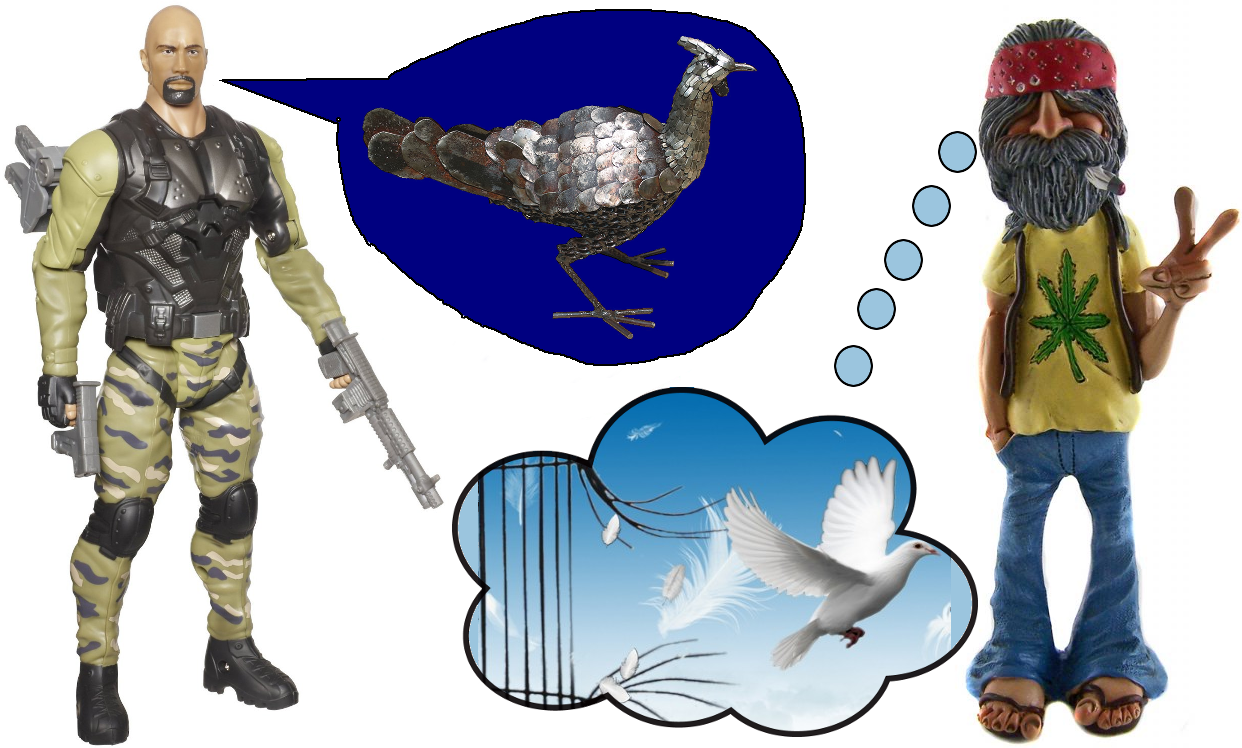
\includegraphics[width=0.9\textwidth]{concepts/usarmy.png}
  \end{figure}
\end{frame}

\begin{frame}{Indestructible ? Donc pas comme ça !}
  \begin{textblock*}{0.25\textwidth}(0.9\textwidth,0.7\textheight)
    
\includegraphics[width=\textwidth]{concepts/trainwestern.png}
  \end{textblock*}
  \centering
  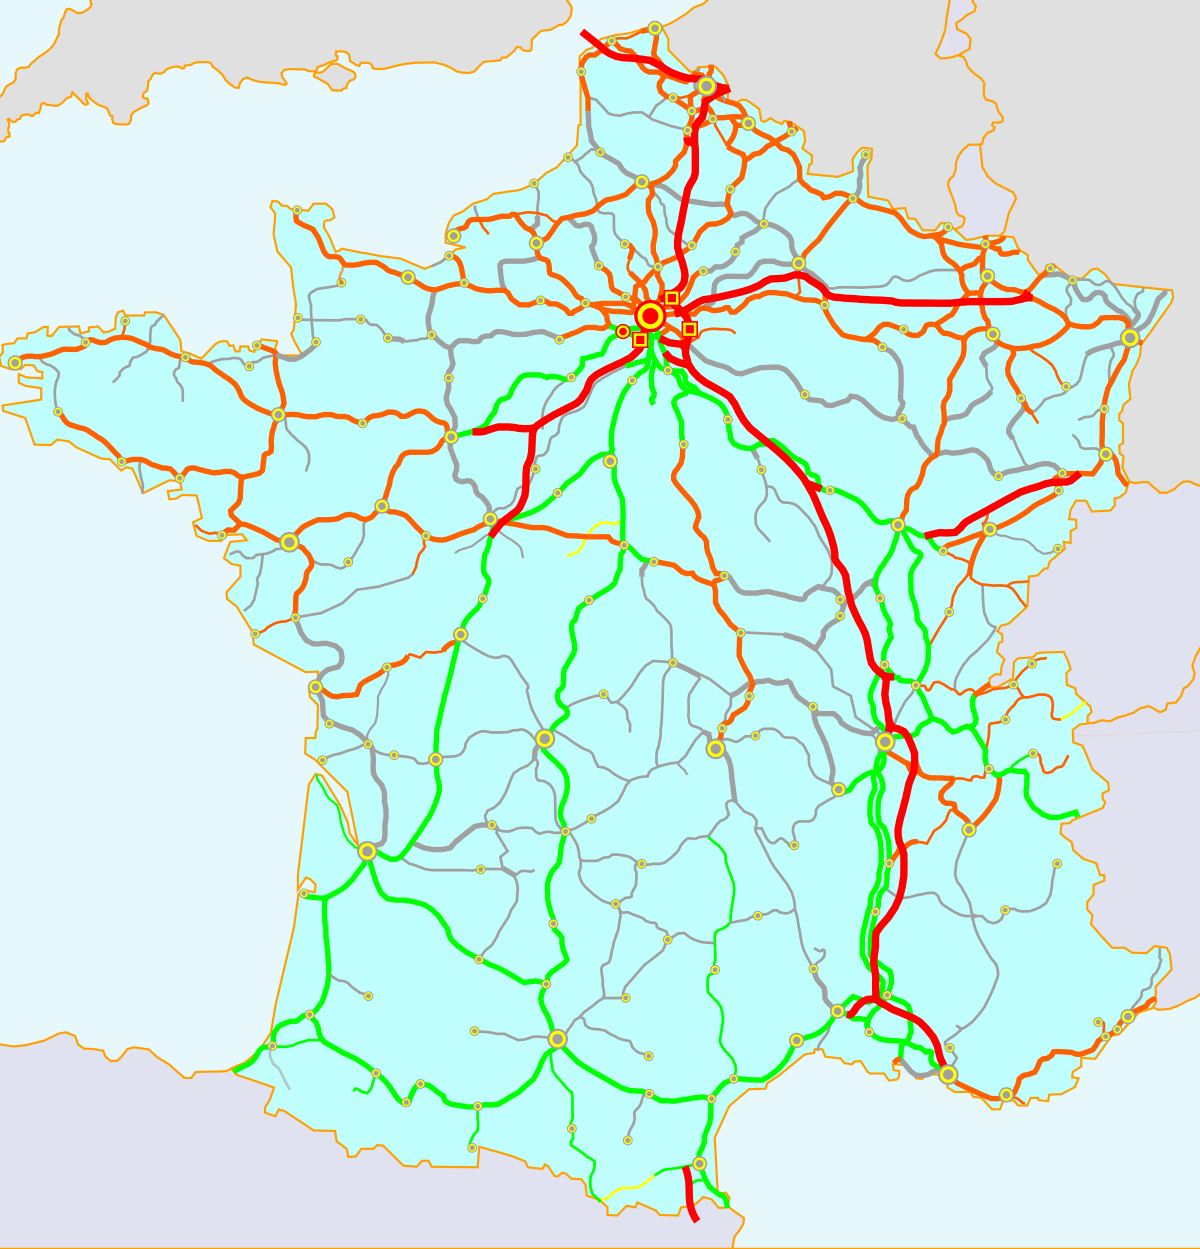
\includegraphics[height=0.8\textheight]{concepts/france.png}
\end{frame}

\begin{frame}{Mais si on en met plusieurs ?}
  \begin{textblock*}{0.25\textwidth}(0.9\textwidth,0.7\textheight)
    
\includegraphics[width=\textwidth]{concepts/trainwestern.png}
  \end{textblock*}
  \centering
  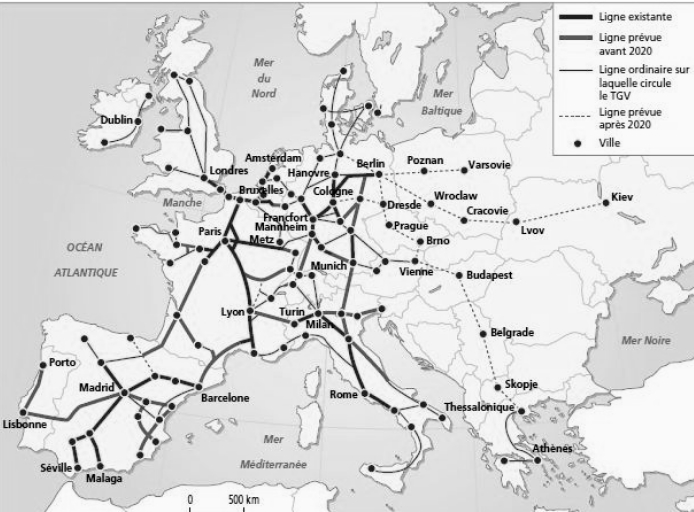
\includegraphics[height=0.8\textheight]{concepts/europe.jpg}
\end{frame}

\subsection{Quelques règles de fonctionnement}

\begin{frame}{Allez, plus en détails :}
  \begin{columns}
  \begin{column}{0.7\textwidth}
    \hspace{5em}Mail\hspace{4em}Web\hspace{3em}P2P
    \vspace{-1em}
    \begin{figure}
      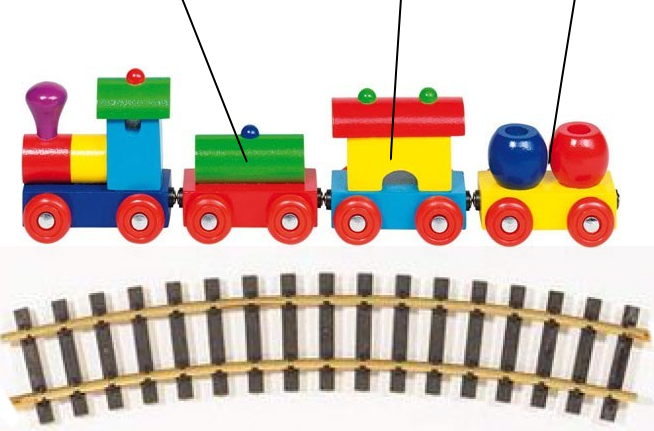
\includegraphics[width=0.9\textwidth]{concepts/protocoles.png}
    \end{figure}
  \end{column}
  \begin{column}{0.4\textwidth}
    \begin{itemize}
      \vspace{2em}
      \item Protocoles et données
      \item Couche IP
      \vspace{2em}
      \item Réseau physique
    \end{itemize}
  \end{column}
  \end{columns}
\end{frame}

\begin{frame}{\hfill(en vrai, il n'y a pas qu'un seul train)}
  \begin{figure}
    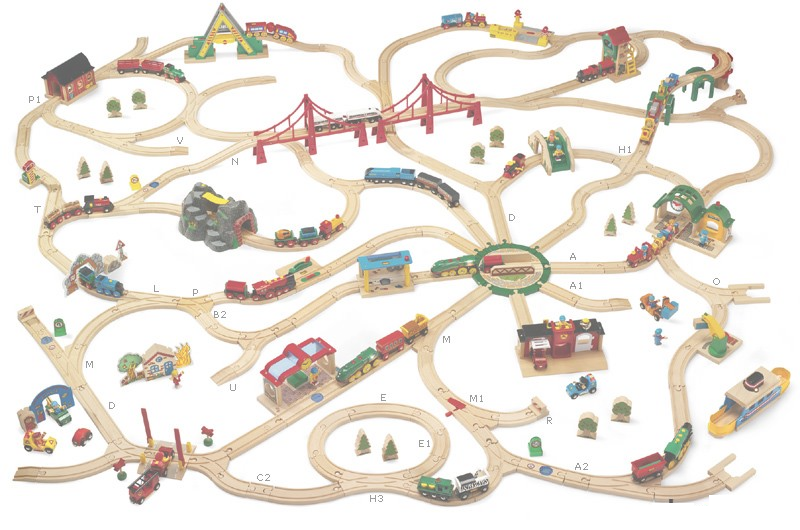
\includegraphics[width=\textwidth]{concepts/rails.png}
  \end{figure}
  \begin{textblock*}{8em}(0.8\textwidth,0.2\textheight)
    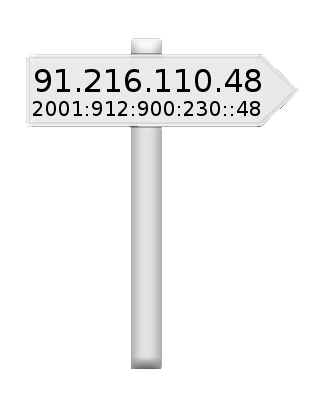
\includegraphics[width=\textwidth]{concepts/ipdirection.png}
  \end{textblock*}
  \begin{textblock*}{12em}(0.3\textwidth,0.3\textheight)
    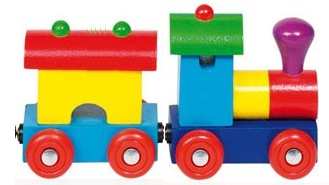
\includegraphics[width=\textwidth]{concepts/paquet.png}
  \end{textblock*}
  \begin{textblock*}{12em}(0.0\textwidth,0.5\textheight)
    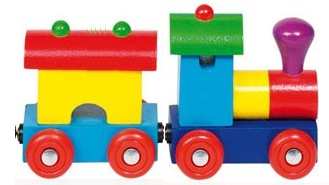
\includegraphics[width=\textwidth]{concepts/paquet.png}
  \end{textblock*}
  \begin{textblock*}{12em}(0.5\textwidth,0.5\textheight)
    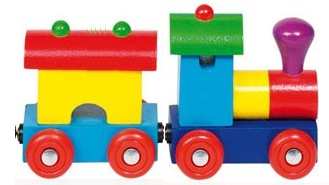
\includegraphics[width=\textwidth]{concepts/paquet.png}
  \end{textblock*}
  \begin{textblock*}{12em}(0.2\textwidth,0.7\textheight)
    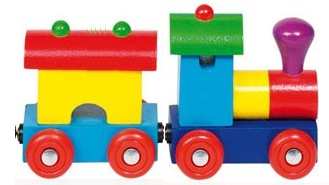
\includegraphics[width=\textwidth]{concepts/paquet.png}
  \end{textblock*}
\end{frame}

\begin{frame}{Une communication par paquets}
  \begin{figure}
    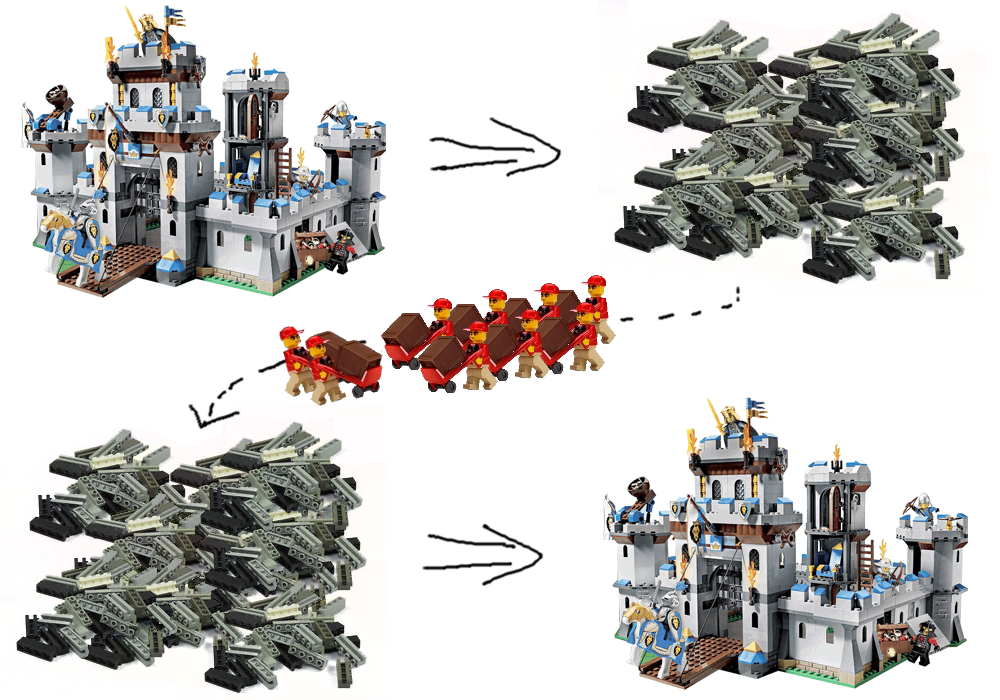
\includegraphics[width=0.9\textwidth]{concepts/lego-paquets.png}
  \end{figure}
\end{frame}

\subsection{Ça donne quoi en pratique ?}

\begin{frame}{Plusieurs routes disponibles…}
  \begin{figure}
    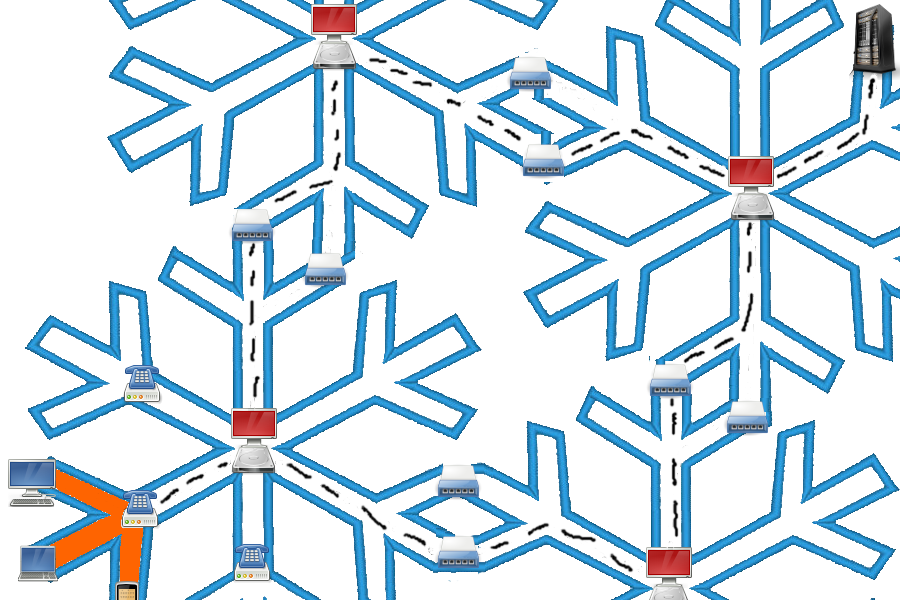
\includegraphics[width=0.9\textwidth]{concepts/flocon-trajet.png}
  \end{figure}
\end{frame}

\begin{frame}{\textit{\textbf{Inter}connection of \textbf{Net}works}}
  \begin{figure}
    \vspace{-0.9em}
    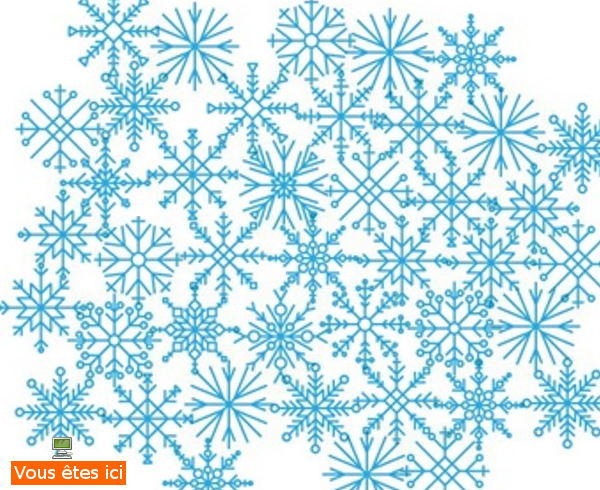
\includegraphics[width=0.9\textwidth]{concepts/flocon-total.png}
  \end{figure}
\end{frame}

\begin{frame}{Si on dessine autrement…}
  \begin{textblock*}{0.28\textwidth}(0.92\textwidth,0.5em)
    
\includegraphics[width=\textwidth]{concepts/rfc1149.png}
  \end{textblock*}
  \includegraphics[width=0.9\textwidth]{concepts/reseau-bazar.png}
\end{frame}

  \section[Les Internets et ses (dérives) d'usages]{Les internets et ses (dérives) d'usages}

\subsection{Les usages d'internets}

\begin{frame}{Concrètement, comment sont utilisés les internets ?}
  \begin{center}
    \includegraphics[height=0.8\textheight]{usages/reseau-bazar.png}
  \end{center}
\end{frame}

\begin{frame}{Concrètement, comment sont utilisés les internets ?}
  \begin{center}
    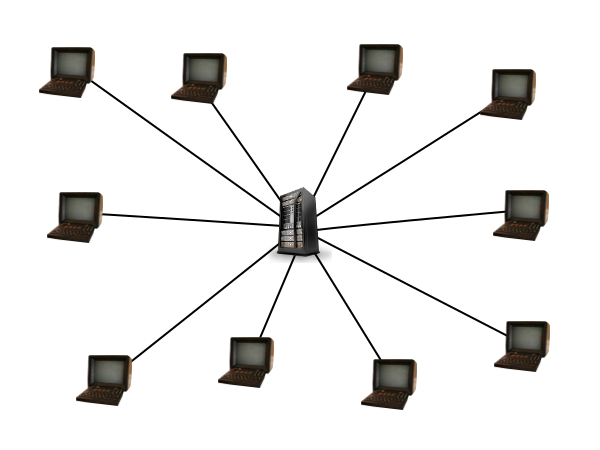
\includegraphics[height=0.8\textheight]{usages/reseau-etoile.png}
  \end{center}
\end{frame}

\subsection{Des dérives "économiques"}

\begin{frame}{Des dérives "économiques"\hfill(1/3)}
  \begin{center}
    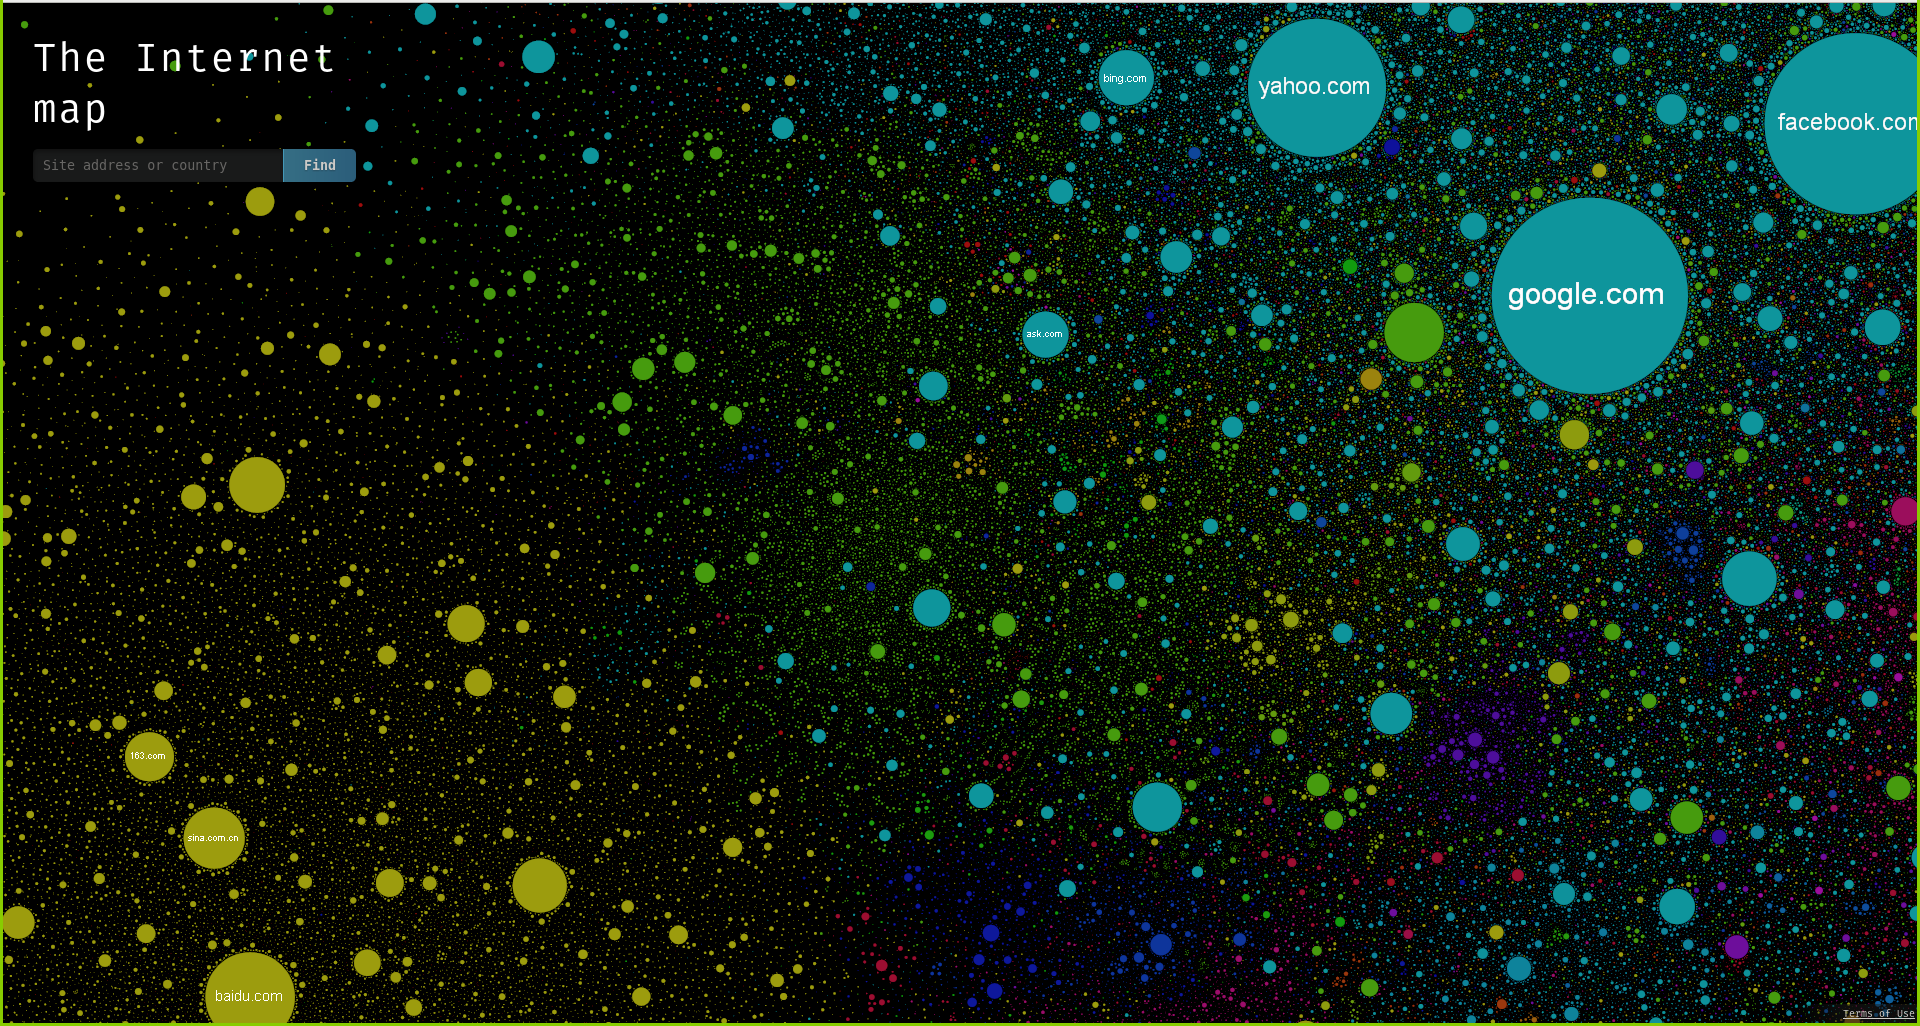
\includegraphics[width=1\textwidth]{usages/internet-map2.png}
  \end{center}
  \footnotesize{\tiny{source: https://internet-map.net}}
\end{frame}

\begin{frame}{Des dérives "économiques"\hfill(2/3)}
  \begin{center}
    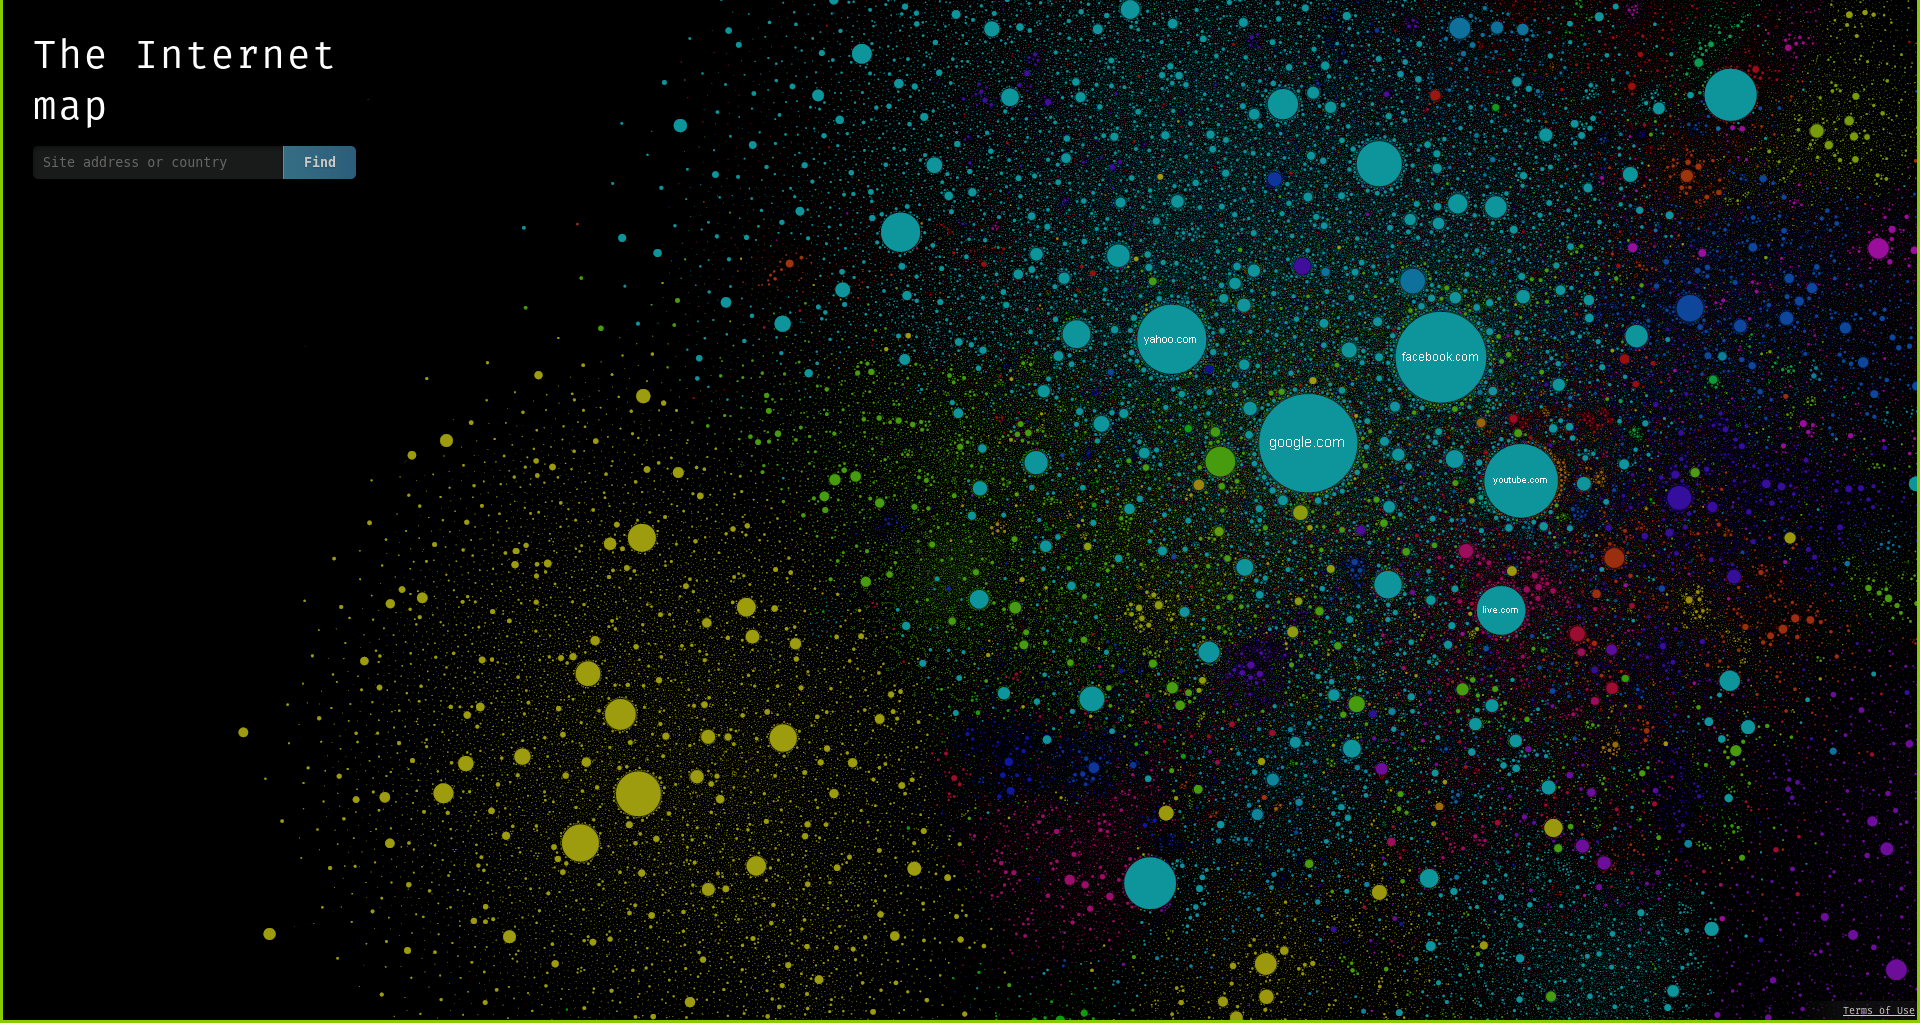
\includegraphics[width=1\textwidth]{usages/internet-map1.png}
  \end{center}
  \footnotesize{\tiny{source: https://internet-map.net}}
\end{frame}

\begin{frame}{Des dérives "économiques"\hfill(3/3)}
  \begin{center}
    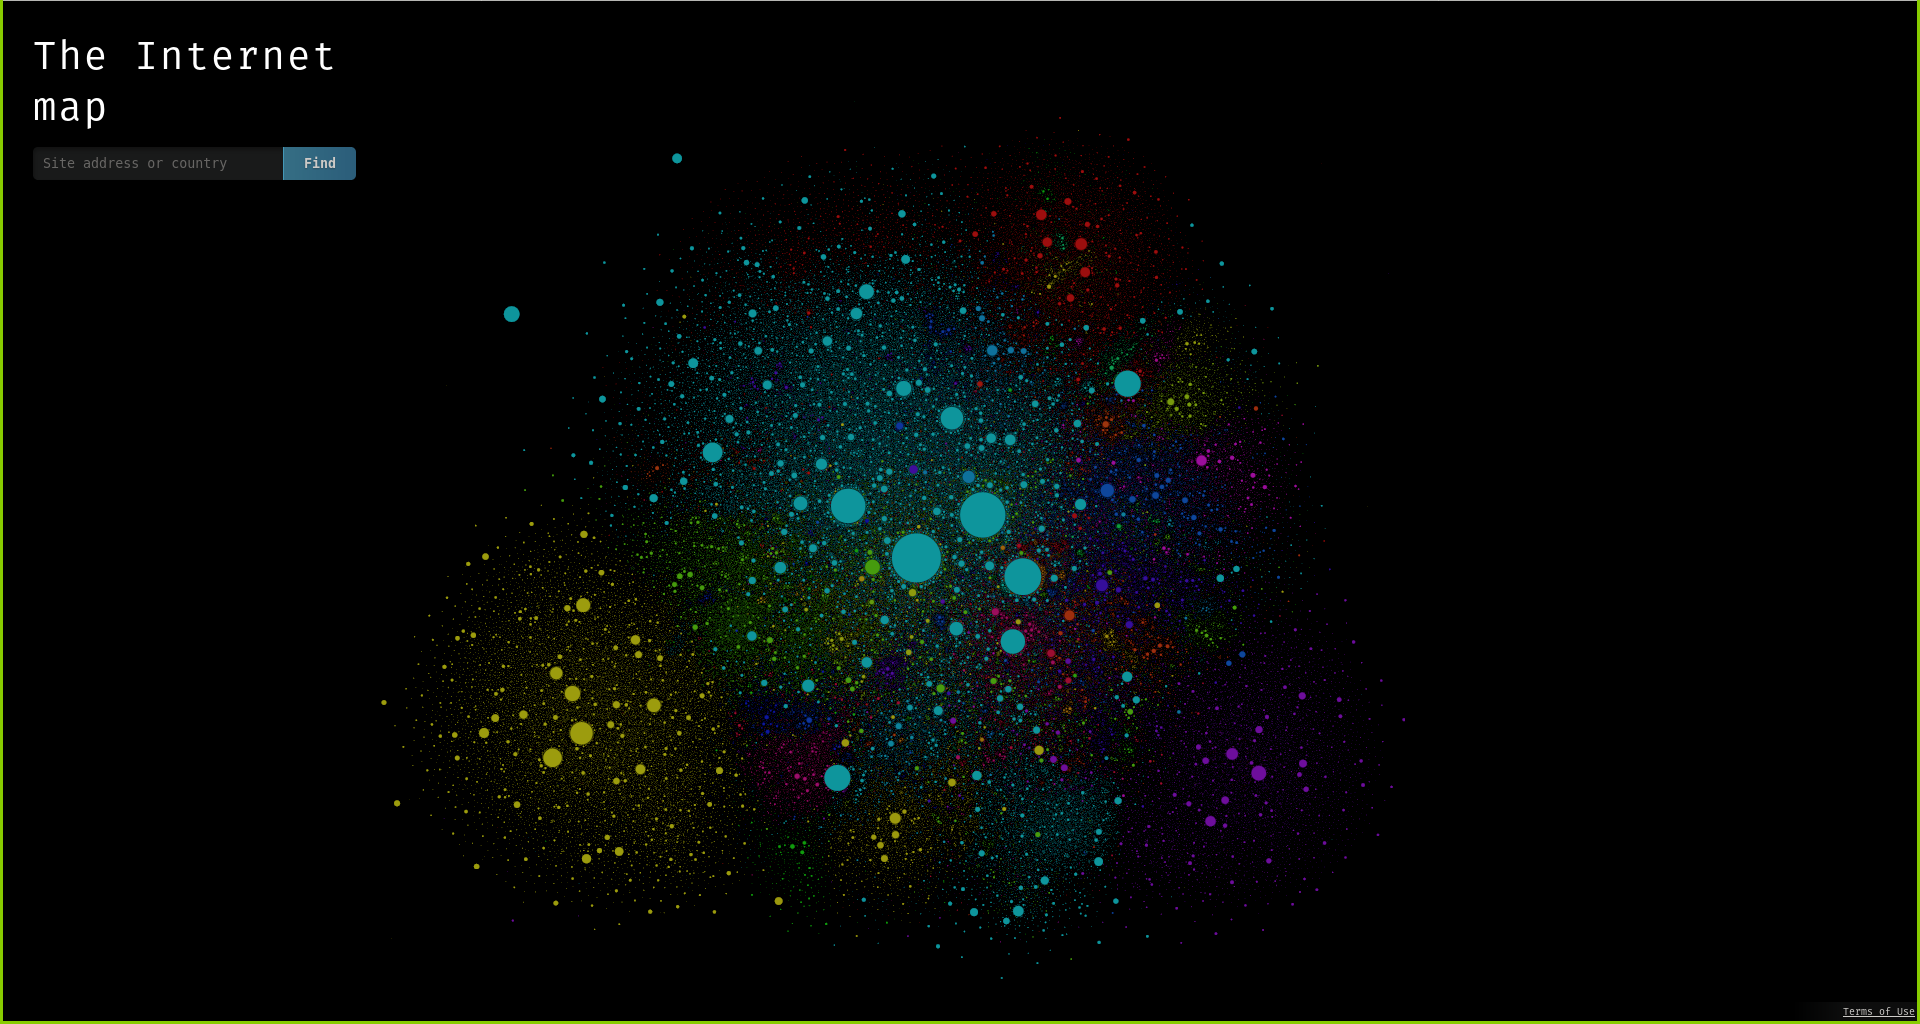
\includegraphics[width=1\textwidth]{usages/internet-map3.png}
  \end{center}
  \footnotesize{\tiny{source: https://internet-map.net}}
\end{frame}

\begin{frame}{Et ce n'est pas QUE la fautes des utilisateurs}
  \begin{columns}
  \begin{column}{0.5\textwidth}
    \raggedright\small
    Les interfaces graphiques:

    \begin{itemize}
      \item Le défilement "infini",
      \item La construction des pages,
      \item La lecture automatique de la vidéo suivante
      \item Et d'autre mécanismes...
    \end{itemize}

    Etudiées et choisies par des humains.
  \end{column}
  \begin{column}{0.5\textwidth}
    \begin{tikzpicture}
      \node (img1) {
\includegraphics[width=.75\textwidth]{usages/scrolling.jpg}};
      \node (img2) at (img1.south east) {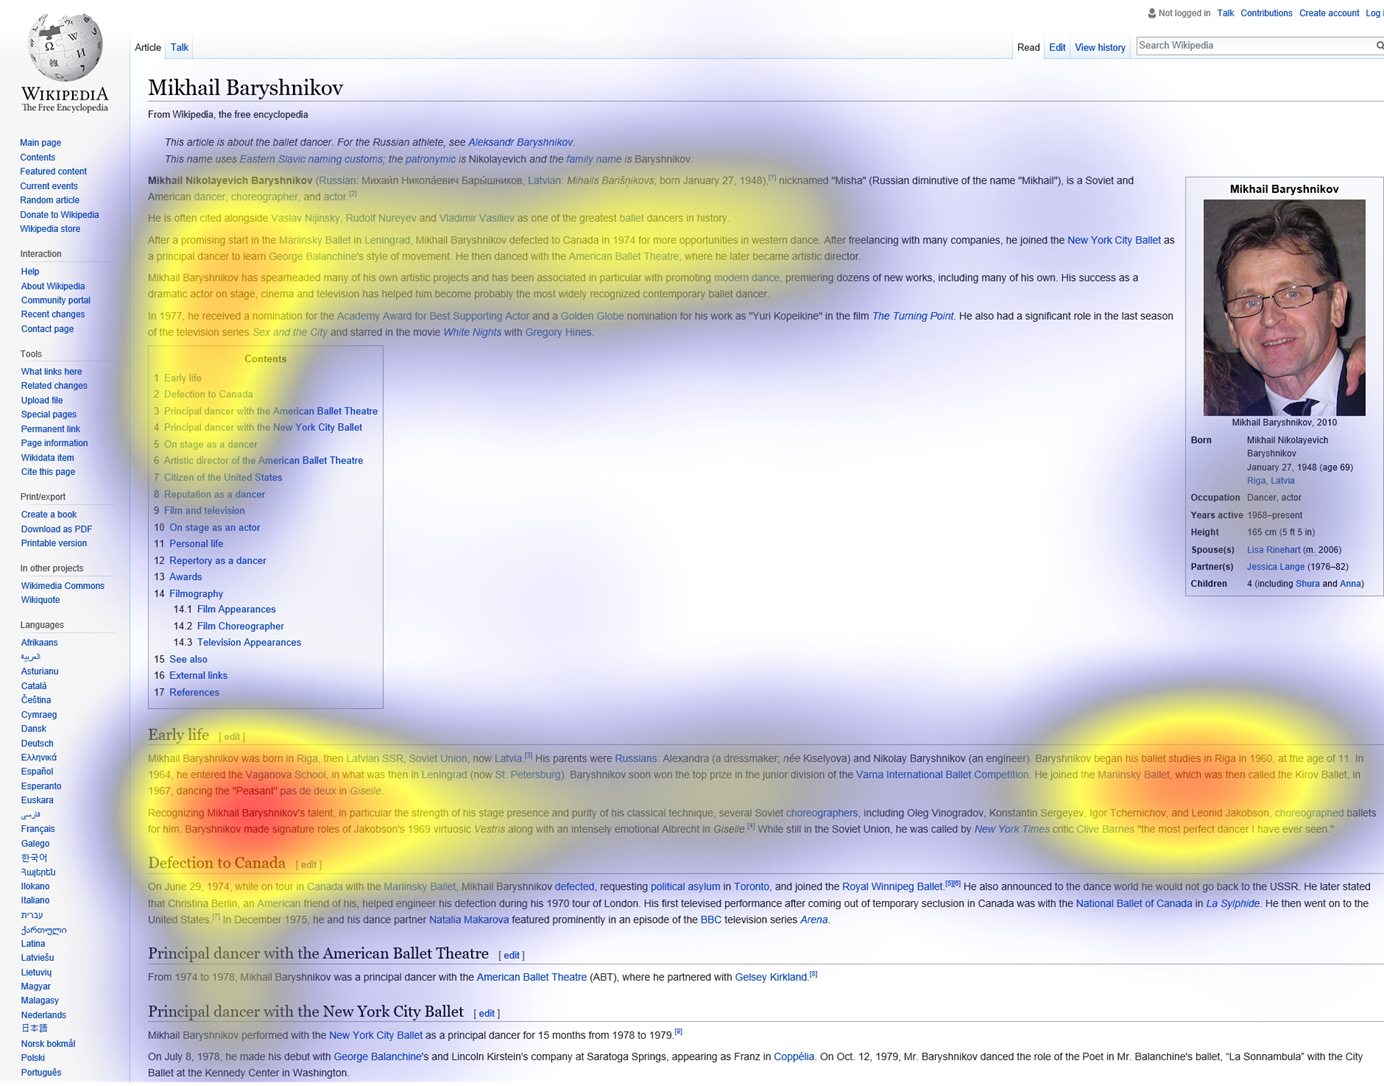
\includegraphics[width=.75\textwidth]{usages/f-pattern.png}};
    \end{tikzpicture}
  \end{column}
  \end{columns}
  \footnotesize{\tiny{source: https://mackeycreativelab.com/about-us/}}\\
  \footnotesize{\tiny{source: https://www.nngroup.com/articles/text-scanning-patterns-eyetracking/}}
\end{frame}


\begin{frame}{"L'intelligence artificielle" et les algorithmes}
    \small
    L'intelligence artificielle n'a rien "d'intelligent" ! \\
    Un algorithme ne décrit qu'une manière de faire, pas comment c'est fait \\
    {\centering
    
\includegraphics[height=0.7\textheight]{usages/intelligence-artificiel.png}\\
    }
  \footnotesize{\tiny{source: https://upload.wikimedia.org/wikipedia/commons/e/ee/Artificial\_Neural\_Network\_with\_Chip.jpg}}
\end{frame}

\begin{frame}{Oui, bon, les GAFAMs, tout ça...}
    \centering
    
\includegraphics[width=0.7\textwidth]{usages/gafam.png}
\end{frame}


\subsection{Des dérives plus "politique"}
\begin{frame}{\hfill ...mais pas que}
  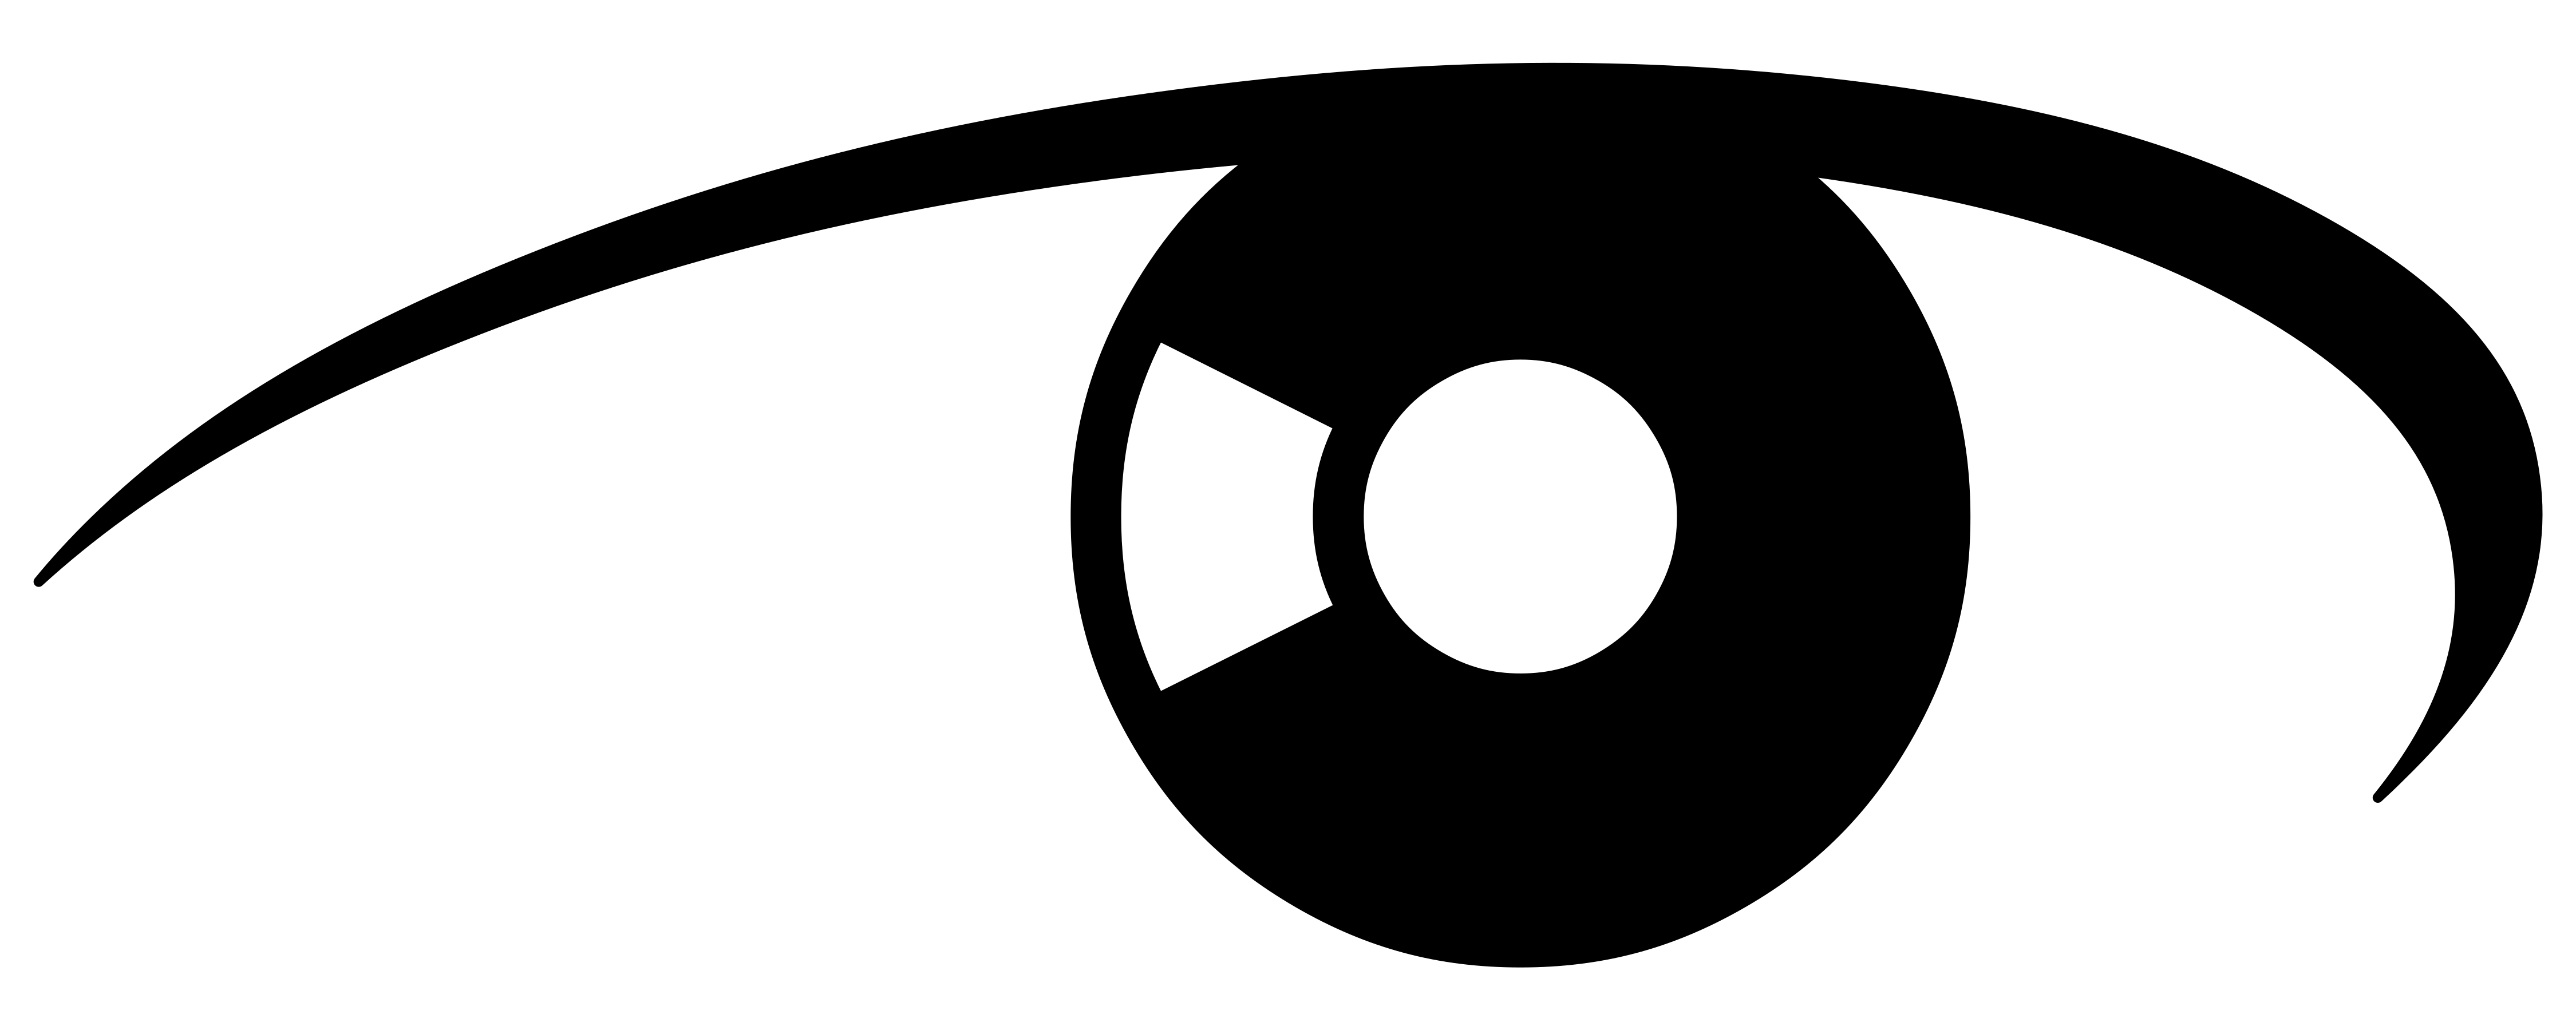
\includegraphics[width=\textwidth]{usages/oeil.png}
\end{frame}

\begin{frame}{La surveillance des espaces publiques}

  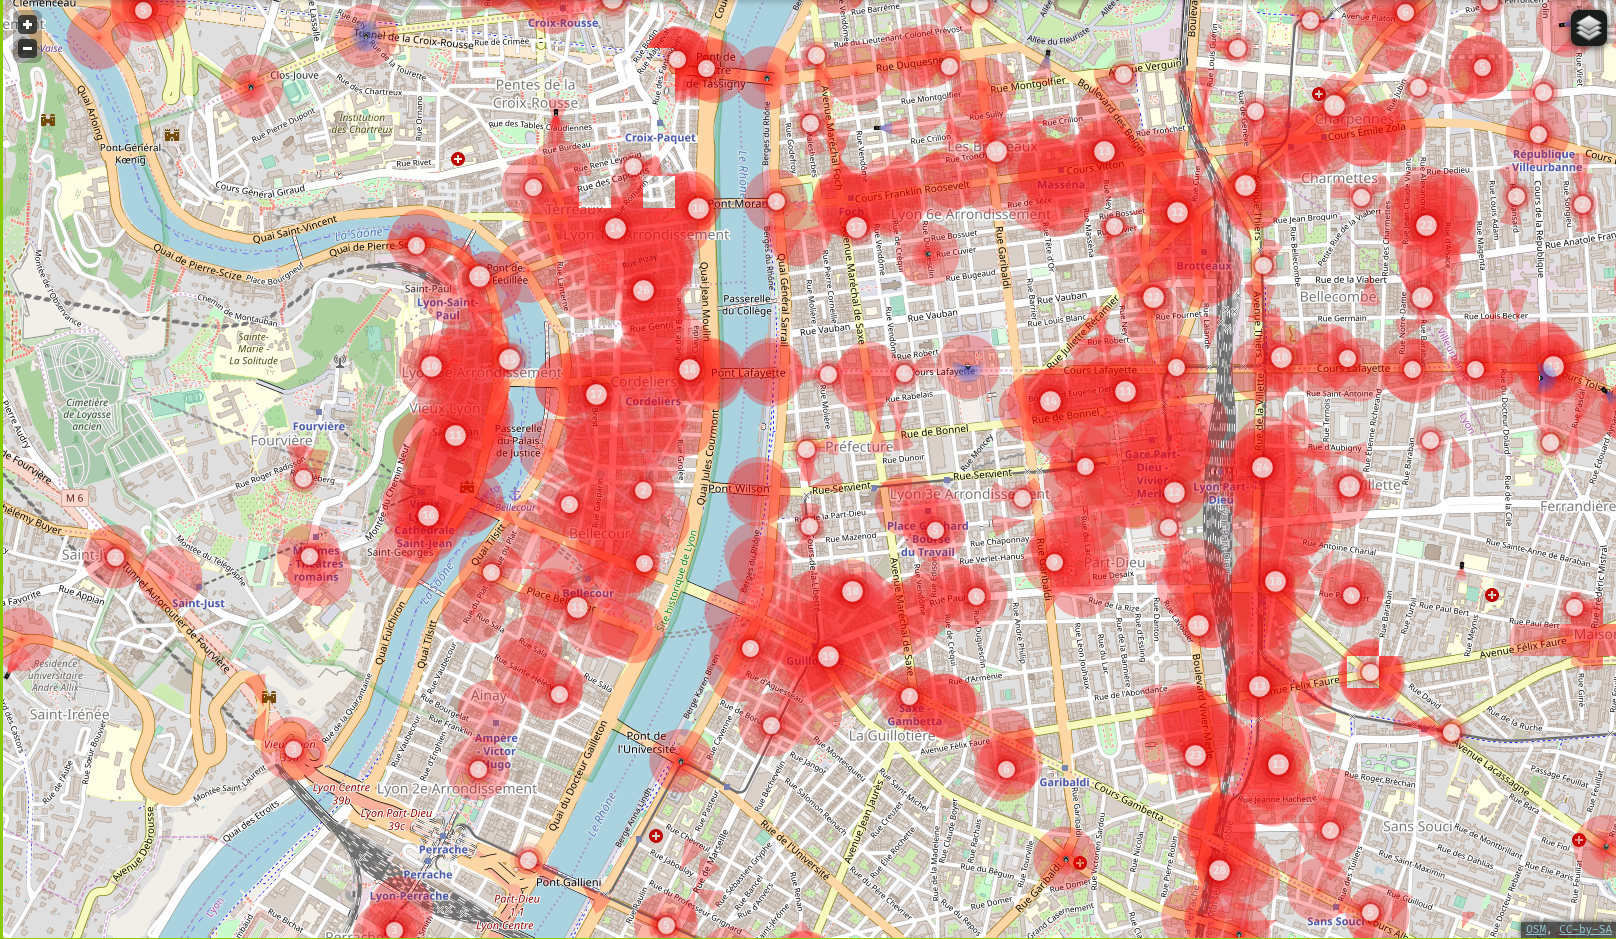
\includegraphics[width=\textwidth]{usages/surveillance_lyon.png}

  Décisions prises par des humains.

  \footnotesize{\tiny{source: https://lyon.sous-surveillance.net/}}
\end{frame}

\begin{frame}{La reconnaissance faciale}
  \tiny
  Expérimentation à Nice et Marseille

  30 Janvier 2020: \\
    - Abandon de l'UE pour l'interdire dans l'espace publique.

  \begin{center}
  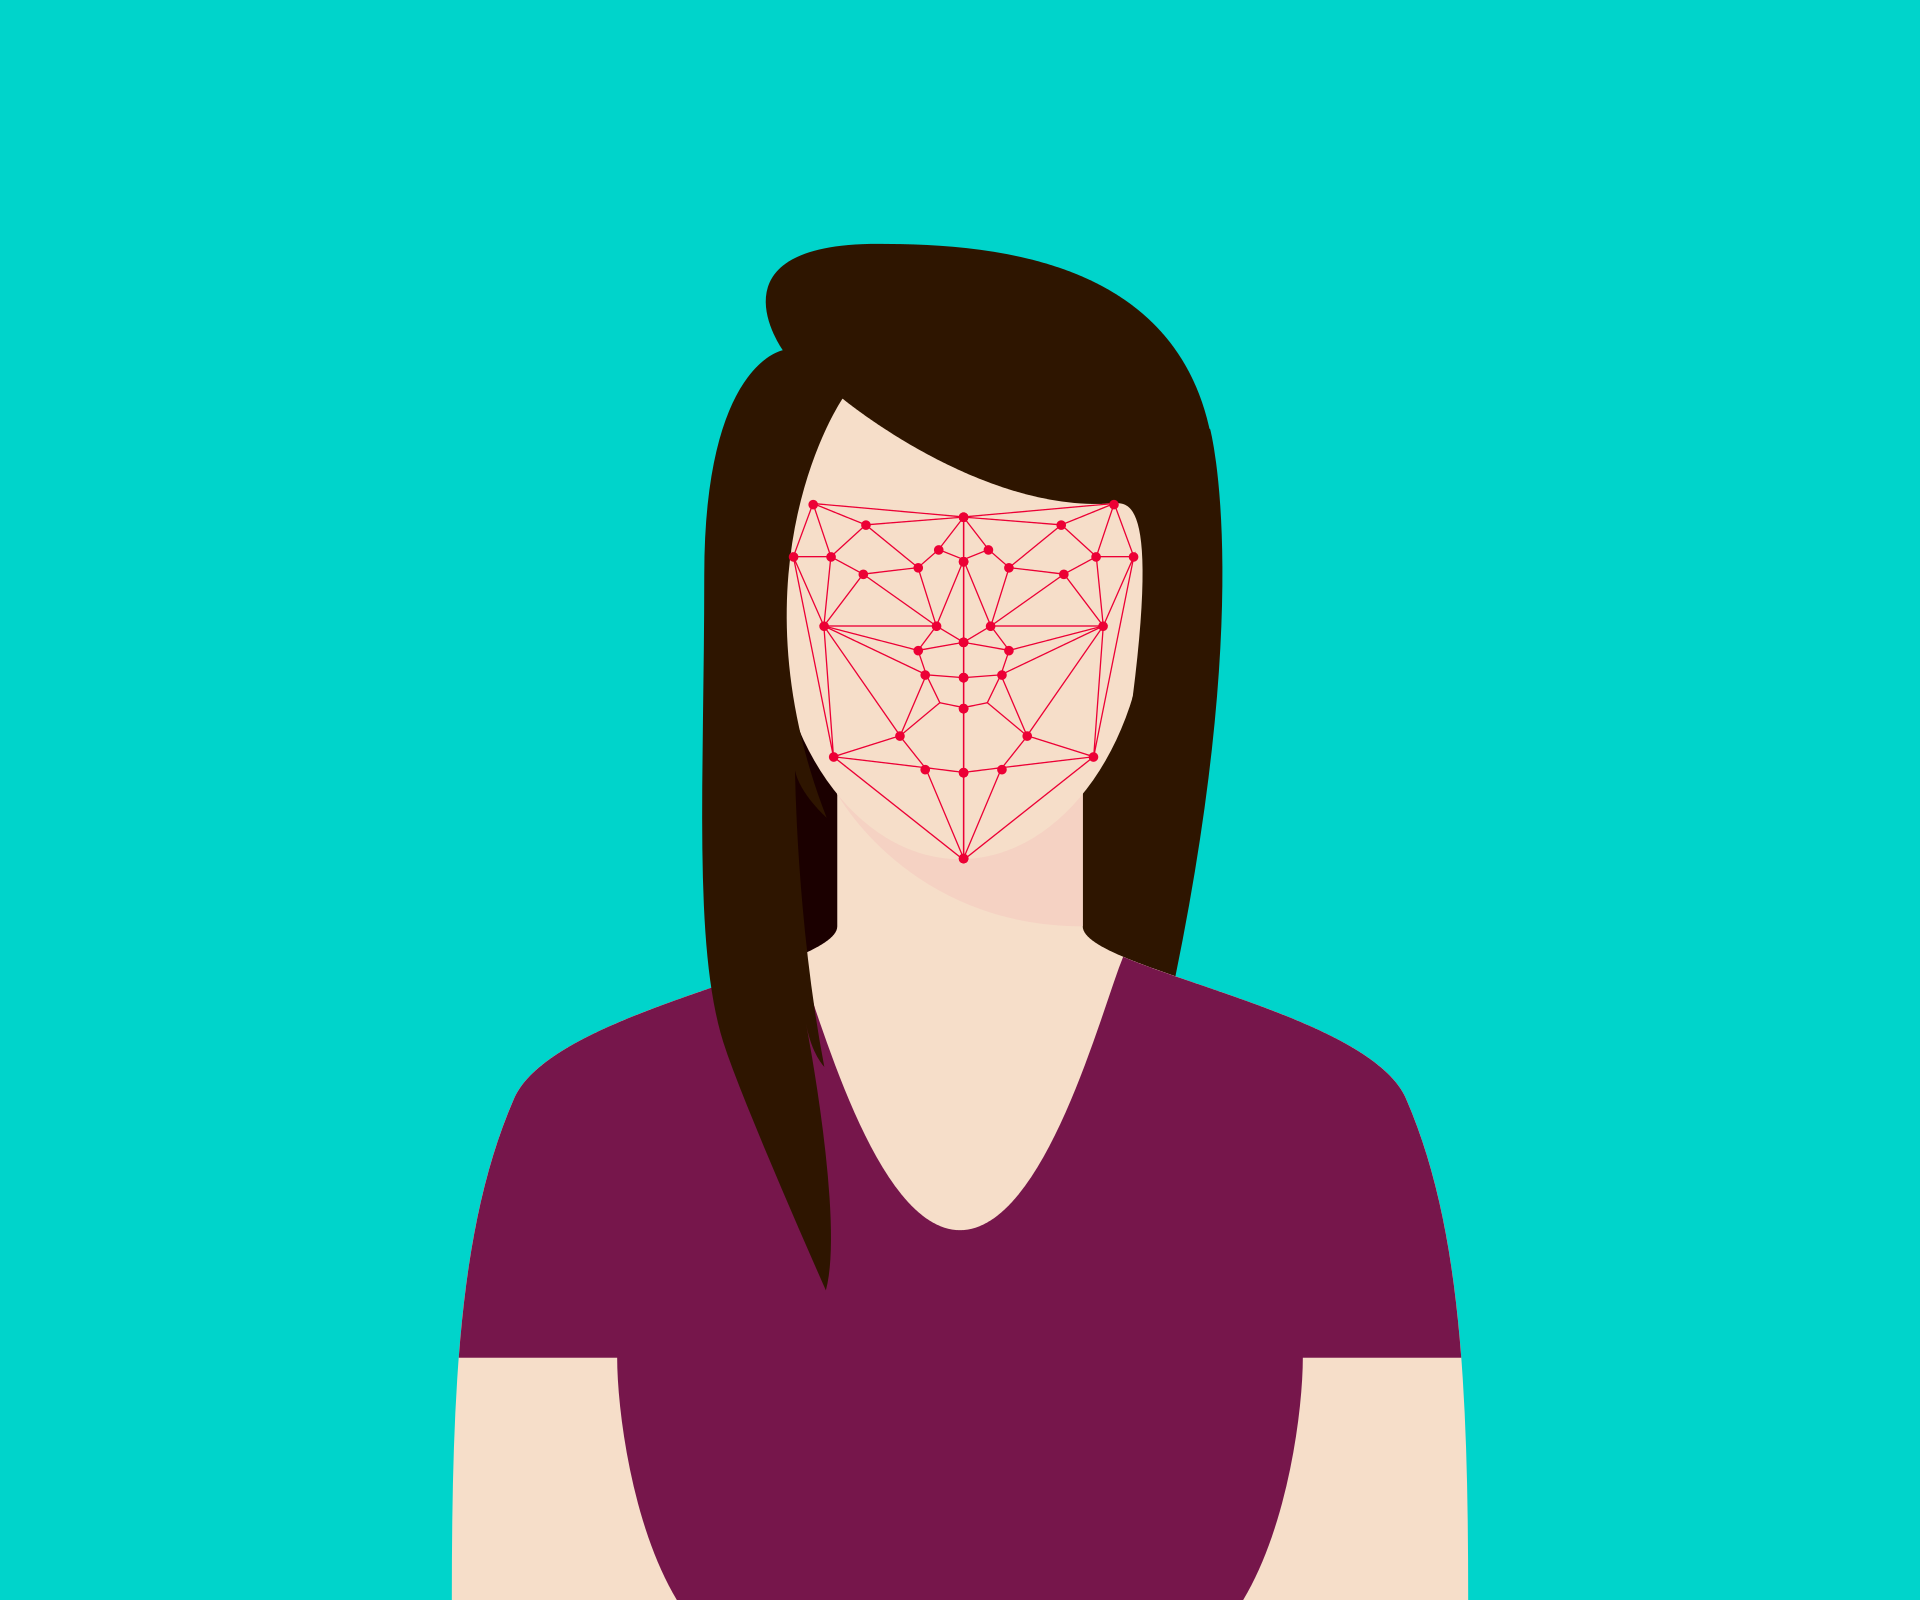
\includegraphics[width=.7\textwidth]{usages/reconnaissance_facial.png}
  \end{center}

  Décisions aussi prises par des humains.
\end{frame}

\begin{frame}{Fiscalité et médias sociaux}
  \small
  Autorisation du FISC français à utiliser les médias sociaux.

  \begin{center}
  
\includegraphics[width=.7\textwidth]{usages/loupe.jpg}
  \end{center}
\end{frame}

\begin{frame}{Système de "Crédit Social"}
  Expérimentation d'un système de réputation des citoyens en chine

  \begin{center}
  
\includegraphics[width=.7\textwidth]{usages/score.jpg}
  \end{center}
\end{frame}

\begin{frame}{Mais et les chats dans tous ça ?}
  \small
  Les internets, ce n'est pas que des machines.\\
  C'est surtout ce que les humains décident d'en faire, à tout les niveaux. \\

  Heureusement, nous pouvons essayer de faire autrement.

  \begin{center}
  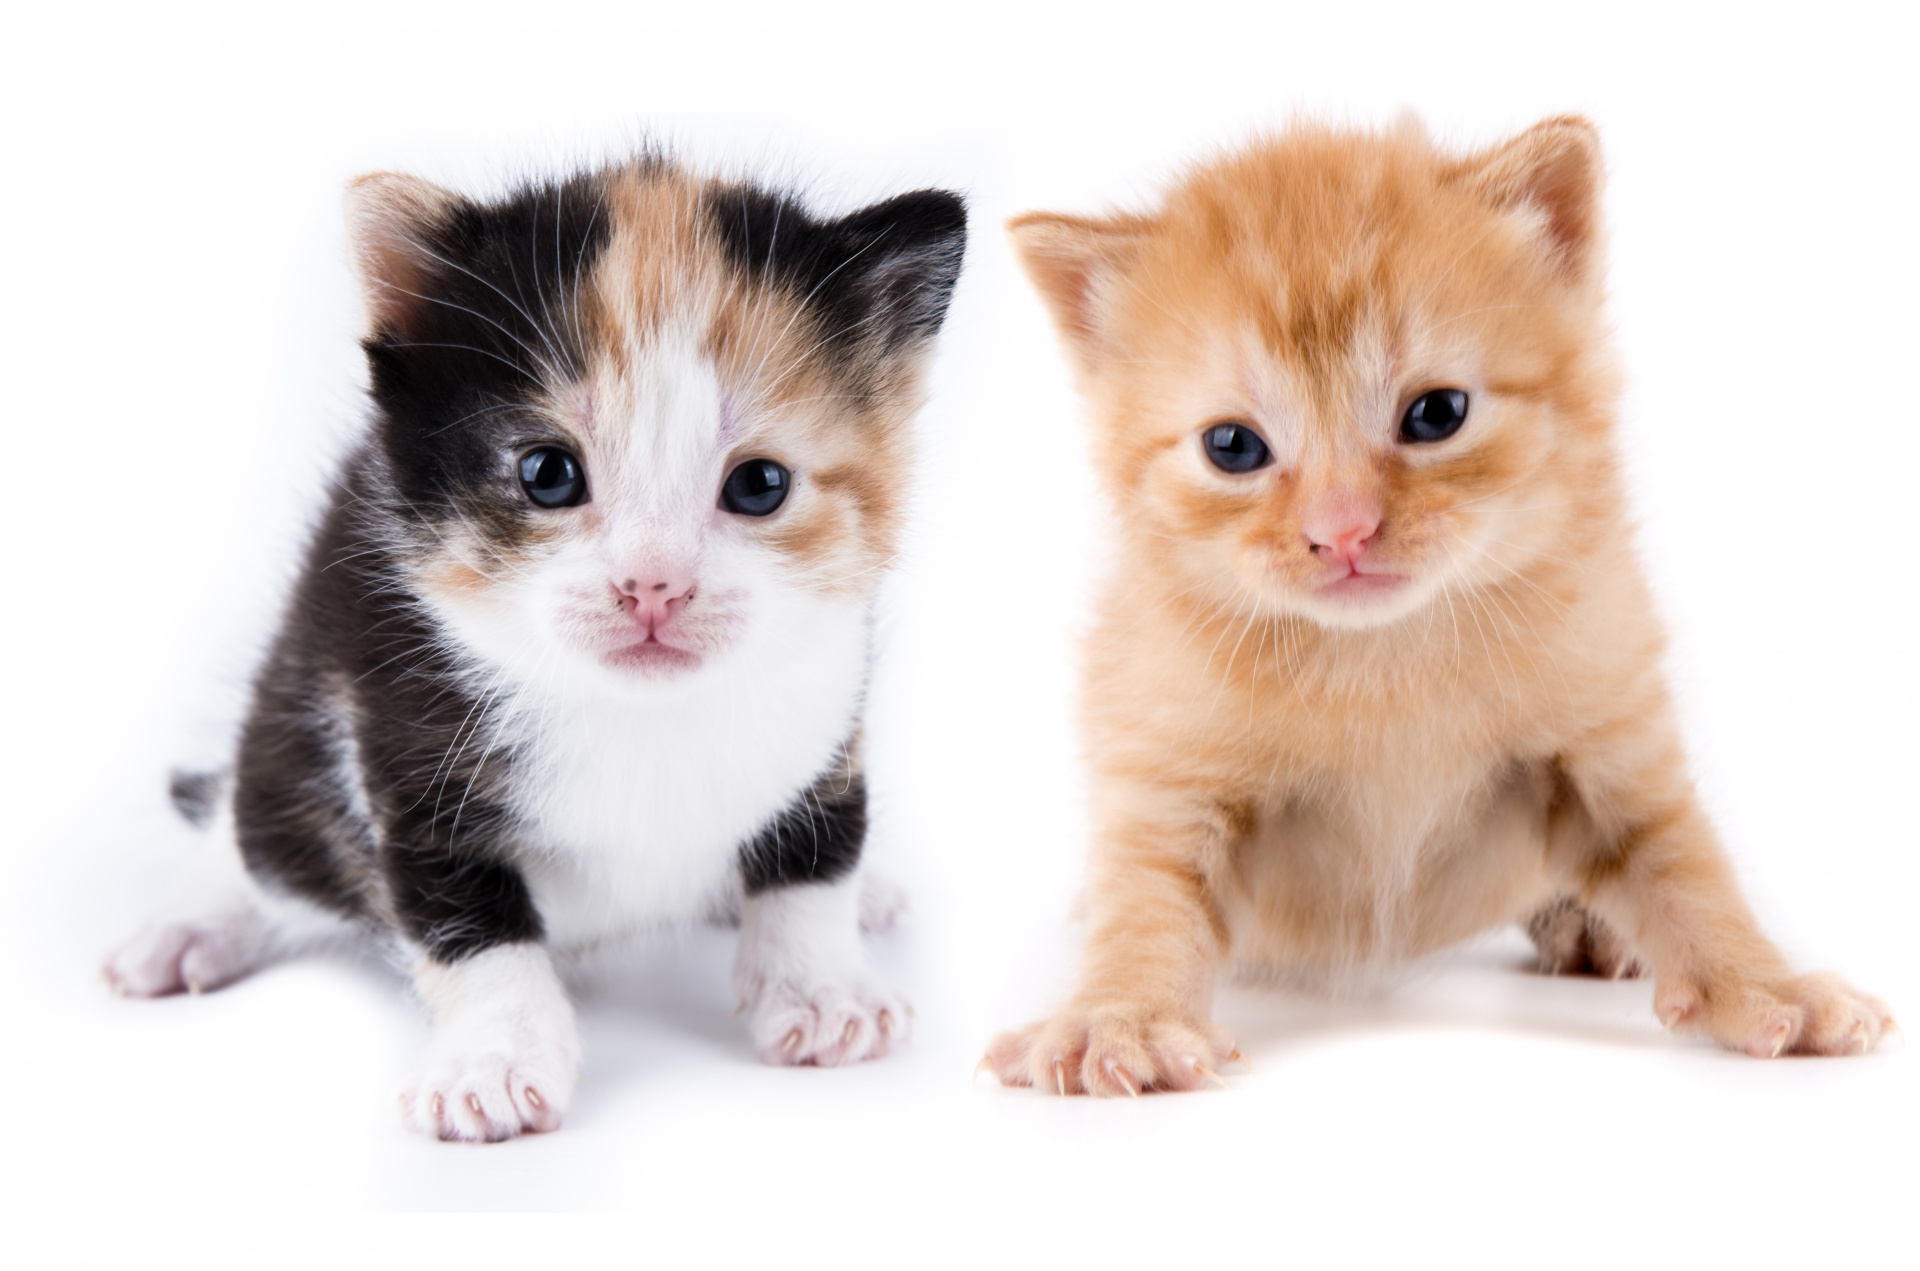
\includegraphics[width=.7\textwidth]{usages/chatons.jpg}
  \end{center}
\end{frame}

% vim: ts=2: sw=2: sts=2





  \section[Plus d'humains, plus de chats, moins de machines]{Plus d'humains, plus de chat, moins de machines}

\subsection{Moins d'algorithmes et plus de contact entre humain}

\begin{frame}{Des acteurs pour des internets plus respectueux (1/2)}
  \begin{center}
    
\includegraphics[height=0.8\textheight]{un_autre_internet/les_fai_dont_vous_etes.pdf}
  \end{center}
\end{frame}

\begin{frame}{Des acteurs pour des internets plus respectueux (2/2)}
  \begin{columns}
    \begin{column}{0.5\textwidth}
      \begin{tabular}{cccc}
        
\includegraphics[width=0.24\textwidth]{un_autre_internet/hadoly.png} &
        \begin{tikzpicture}
          \node (img1) at (0,0) {
\includegraphics[width=0.24\textwidth]{un_autre_internet/arn.png}};
          \node (img2) at (0, -1) {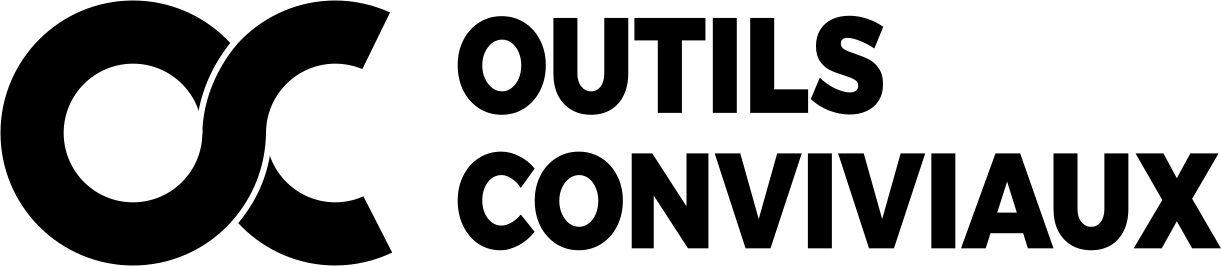
\includegraphics[width=0.24\textwidth]{un_autre_internet/outils_conviviaux.png}};
        \end{tikzpicture} &
        
\includegraphics[width=0.24\textwidth]{un_autre_internet/tux_family.png} &
        
\includegraphics[width=0.24\textwidth]{un_autre_internet/framasoft.png}  \\
        
\includegraphics[width=0.24\textwidth]{un_autre_internet/marsnet.png} &
        
\includegraphics[width=0.24\textwidth]{un_autre_internet/devloprog.png} &
        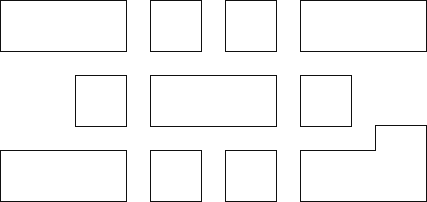
\includegraphics[width=0.24\textwidth]{un_autre_internet/3hg.png} &
        
\includegraphics[width=0.24\textwidth]{un_autre_internet/artifaille.png} \\
      \end{tabular}
    \end{column}
    \begin{column}{0.5\textwidth}
    \begin{center}
      \includegraphics[height=0.8\textheight]{un_autre_internet/chatons.png}
    \end{center}
    \end{column}
  \end{columns}
\end{frame}

\begin{frame}{Des volontés communes}
  \begin{columns}
    \begin{column}{0.4\textwidth}
      \begin{itemize}
        \item La neutralité du net
        \item La transparence
        \item L'humain au centre
        \item Rester local
      \end{itemize}
    \end{column}
    \begin{column}{0.6\textwidth}
      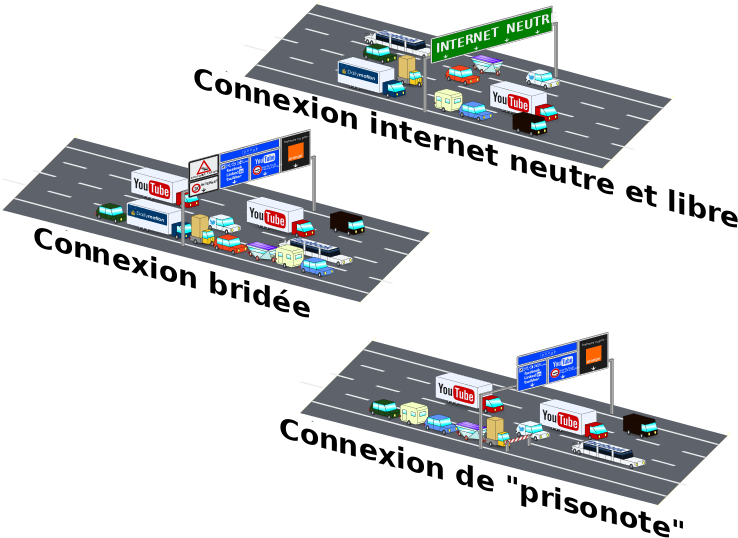
\includegraphics[width=0.4\textwidth]{un_autre_internet/autoroute.png}
      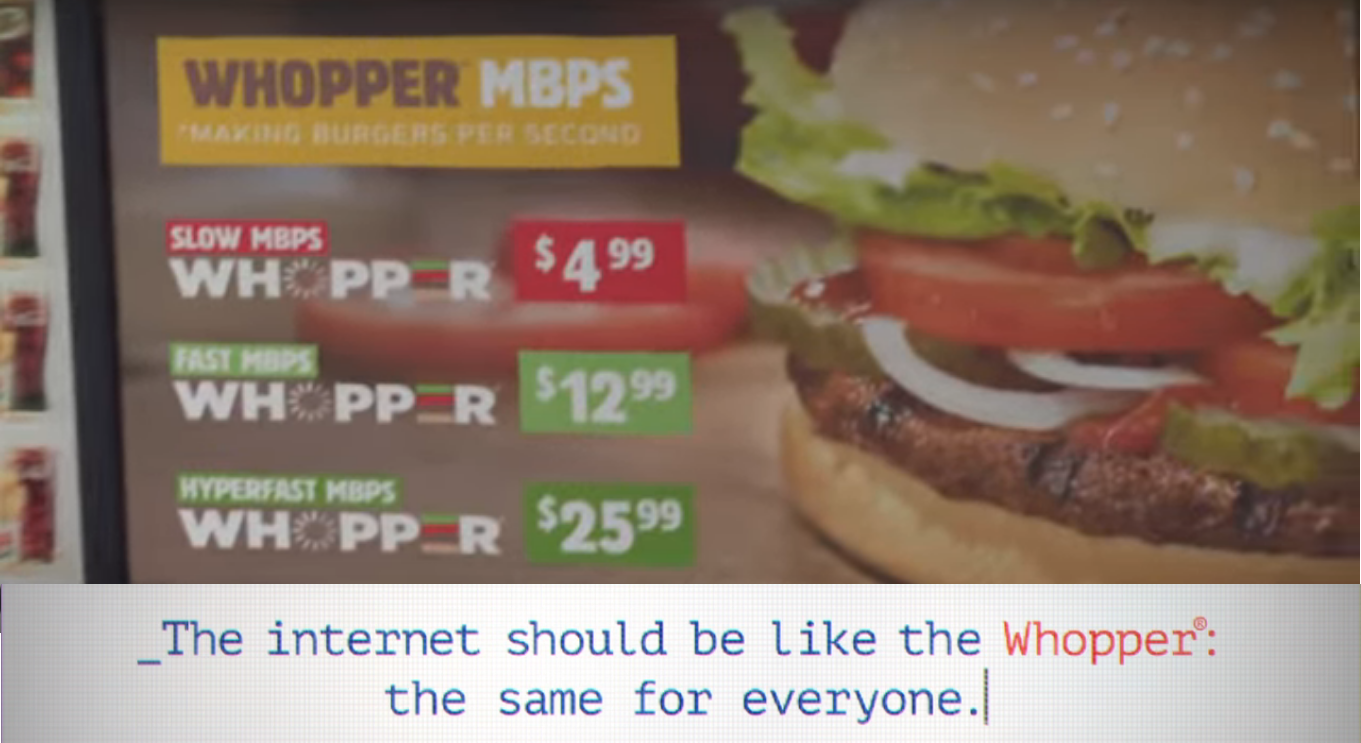
\includegraphics[width=0.4\textwidth]{un_autre_internet/whopper.png} \\
      
\includegraphics[width=0.4\textwidth]{un_autre_internet/local.png}
      
\includegraphics[width=0.4\textwidth]{un_autre_internet/groupetravail.png}
    \end{column}
  \end{columns}
\end{frame}

\subsection{Les CHATONS: Hadoly}

\begin{frame}{Hadoly: Hébergeur Associatif Décentralisé et Ouvert à Lyon}
  \begin{columns}
    \begin{column}{0.5\textwidth}
      \centering
      
\includegraphics[width=0.5\textwidth]{un_autre_internet/hadoly.png}\\
      https://hadoly.fr/
    \end{column}
    \begin{column}{0.5\textwidth}
      \begin{itemize}
        \item Services ouverts à tous
        \begin{itemize}
            \item Pads
            \item Wiki
            \item Docs
            \item PostIt
        \end{itemize}
        \item Services aux adhérents
        \begin{itemize}
          \item Mail
          \item Cloud
          \item Git
          \item Projets
        \end{itemize}
      \end{itemize}
    \end{column}
  \end{columns}
\end{frame}

\begin{frame}{Hadoly: Des services ouverts à tous}
  \centering
  \includegraphics[width=0.8\textwidth]{un_autre_internet/pad_hadoly.png}\\
\end{frame}

\begin{frame}{Hadoly: C'est aussi des mails}
  \centering
  \includegraphics[width=0.8\textwidth]{un_autre_internet/rainloop.png}\\
  \tiny Image presque contractuelle.
\end{frame}

\begin{frame}{Hadoly: Un espace de stockage en ligne ("cloud")}
  \centering
  \includegraphics[width=0.8\textwidth]{un_autre_internet/nextcloud.png}\\
  \tiny Image presque contractuelle.
\end{frame}

\begin{frame}{Hadoly: Et bien d'autres}
  \centering
  \begin{tikzpicture}
    \node (img1) {\includegraphics[width=0.7\textwidth]{un_autre_internet/kanboard.png}};
    \node (img2) at (img1.south east) {\includegraphics[width=0.7\textwidth]{un_autre_internet/gitea.png}};
  \end{tikzpicture}\\
  \tiny Images presque contractuelles.
\end{frame}

\subsection{Les FAI Associatif: Illyse}

\begin{frame}{Illyse: Internet Libre sur Lyon et Saint-Etienne}
  \begin{columns}
    \begin{column}{0.5\textwidth}
      \centering
      \includegraphics[width=0.8\textwidth]{un_autre_internet/illyse.png}\\
      https://www.illyse.net/
    \end{column}
    \begin{column}{0.5\textwidth}
      \begin{itemize}
        \item De l'xDSL
        \item Des VPNs
        \item De l'internet par onde radio
        \item De la fibre \\{\tiny(pour l'instant, dans la Loire)}
      \end{itemize}
    \end{column}
  \end{columns}
\end{frame}

\begin{frame}{Illyse: De l'xDSL ...}
  \centering
  \includegraphics[width=0.8\textwidth]{un_autre_internet/adsl.png}
\end{frame}

\begin{frame}{Illyse: \hfill ... Du VPN ...\hfill}
  \centering
  \includegraphics[width=0.8\textwidth]{un_autre_internet/vpn.png}
\end{frame}

\begin{frame}{Illyse: \hfill ... De l'internet par onde radio ...\hfill}
  \centering
  \includegraphics[width=0.8\textwidth]{un_autre_internet/antennes.png}
\end{frame}

\begin{frame}{Illyse: \hfill ... Et de la fibre (1/2)}
  \begin{columns}
    \begin{column}{0.5\textwidth}
      \centering
      \includegraphics[width=0.4\textwidth]{un_autre_internet/fibre_1.png}
      \includegraphics[width=0.4\textwidth]{un_autre_internet/fibre_2.png}\\
      \includegraphics[width=0.4\textwidth]{un_autre_internet/fibre_3.png}
    \end{column}
    \begin{column}{0.5\textwidth}
      \centering
      \includegraphics[width=\textwidth]{un_autre_internet/fibre_zone_dense.png}
    \end{column}
  \end{columns}
\end{frame}

\begin{frame}{Illyse: \hfill ... Et de la fibre (2/2)}
  \centering
  Donc si j'habite dans la loire ?
  \includegraphics[width=0.8\textwidth]{un_autre_internet/fibre_yeah.png} \\
  Sinon, malheureusement, il va falloir attendre.
\end{frame}


\begin{frame}{Convaincu·e·s ? Alors rejoignez-nous}
  \centering
  Faisons des internets un monde plus humains, \\
  mais avec toujours autant de chats !

  \includegraphics[height=0.7\textheight]{un_autre_internet/adoptez_les.png}
\end{frame}

% vim: ts=2: sw=2: sts=2

  \setcounter{framenumber}{42}
\end{document}
